\documentclass[biblatex]{deltares_memo}

\newcommand{\netcdf}{netCDF\xspace}
\newcommand{\ugrid}{UGRID\xspace}

\begin{document}
\memoTo{Participants of the Danubius-RI modelling hackaton}
\memoConfidentialUntil{}
\memoDate{\today~\currenttime}
\memoVersion{001}
\memoFrom{Jan Mooiman}
\memoTelephone{+31\,(0)88\,335\,8568}
\memoEmail{jan.mooiman@deltares.nl}
\memoSubject{Some explanation of the layout of the UGRID example files}
\memoCopy{}

\deltarestitle
%------------------------------------------------------------------------------
\section{Introduction}

In the following two sections the layout and numbering of node, edge and faces is presented of the meshes which are generated by the python-scripts:
\begin{enumerate}
	\item \texttt{ugrid\_2d\_map\_triangles.py} and
	\item \texttt{ugrid\_2d\_map\_quadrangles.py}
\end{enumerate}

The python script \texttt{ugrid\_2d\_map\_triangles.py} will generate a \ugrid \netcdf file with a mesh as shown in \autoref{sec:triangles}.
This mesh contains only triangles.

The python script \texttt{ugrid\_2d\_map\_quadrangles.py} will generate a \ugrid \netcdf file with a mesh as shown in \autoref{sec:quadrangles}. 
This mesh contains triangles as well as quadrangles.
The variable names in this example python script are replaced anonymous names, called \texttt{name$\ast$}.

The numbering in the pictures is 1-based. Which is indicated by the suffix "\textbf{:1}" behind the count number.
%------------------------------------------------------------------------------
\section{Mesh consisting of only triangles \label{sec:triangles}}
\begin{figure}[H]	
	\centering
	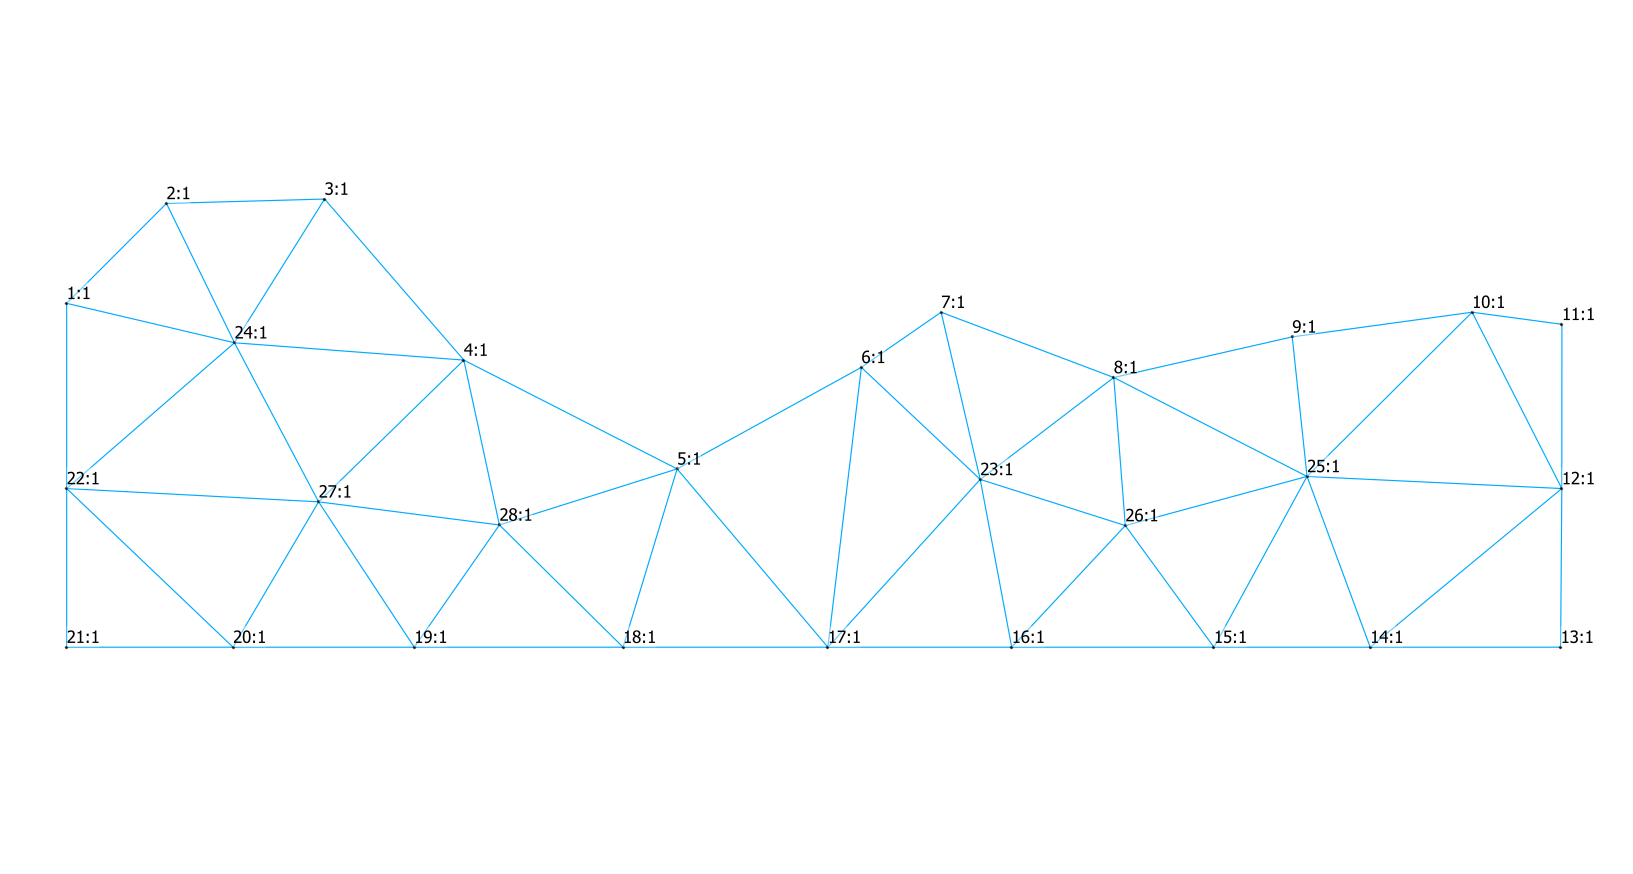
\includegraphics[width=0.8\textwidth]{pictures/node_numbers_triangles.png}
	\caption{Node numbers (1-based) of mesh consisting of only triangles}
\end{figure}
\begin{figure}[H]	
	\centering
	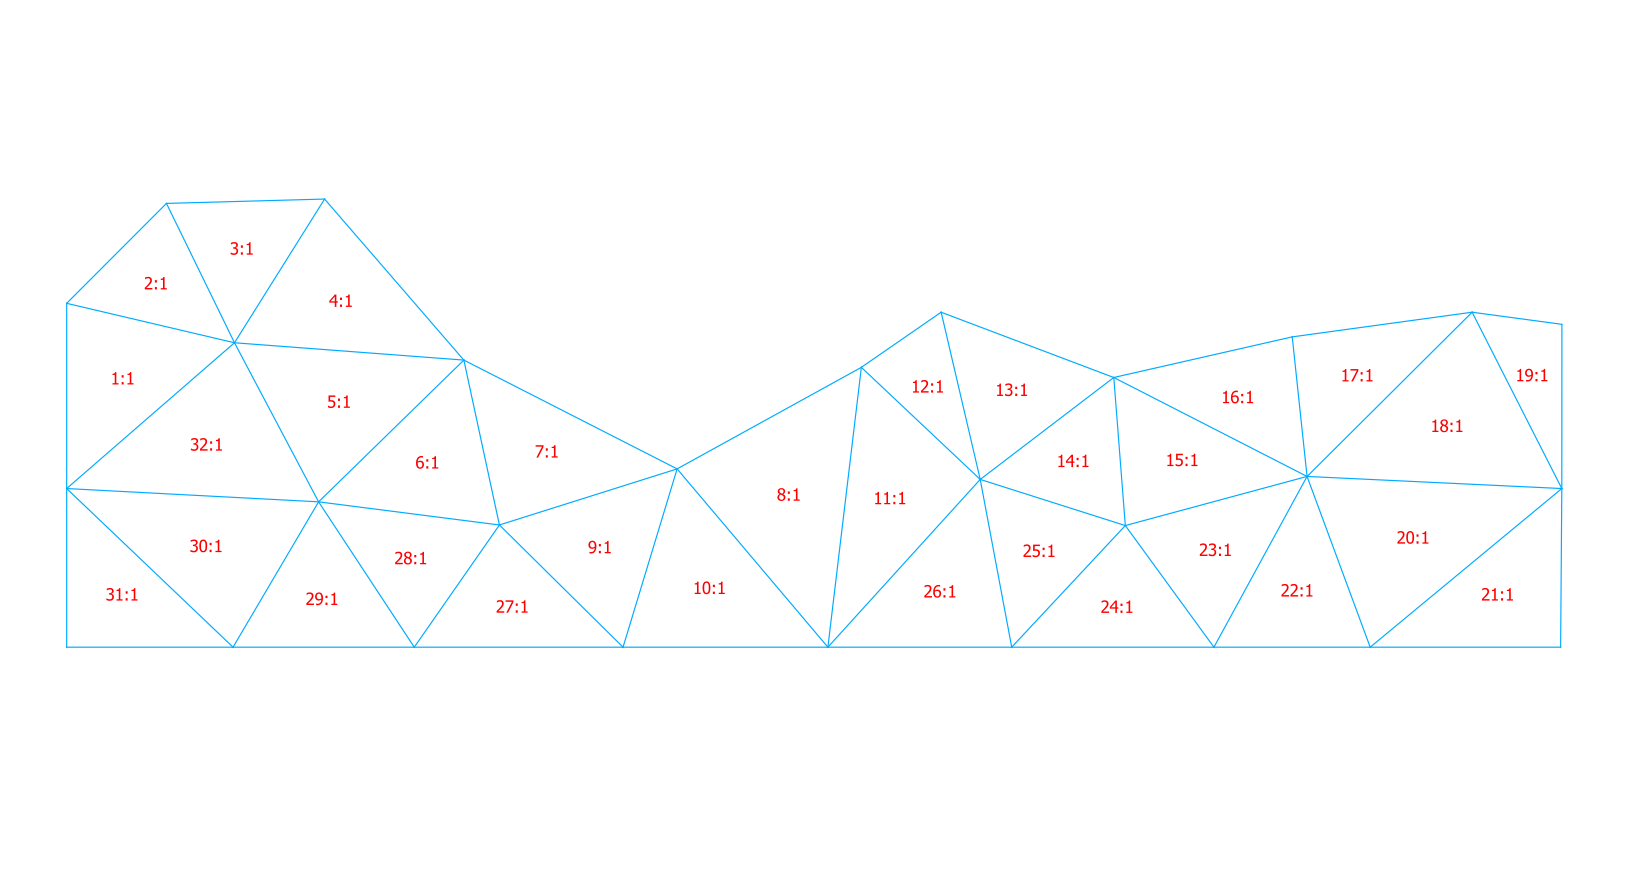
\includegraphics[width=0.8\textwidth]{pictures/face_numbers_triangles.png}
	\caption{Face numbers (1-based) of mesh consisting of only triangles}
\end{figure}
\begin{figure}[H]	
	\centering
	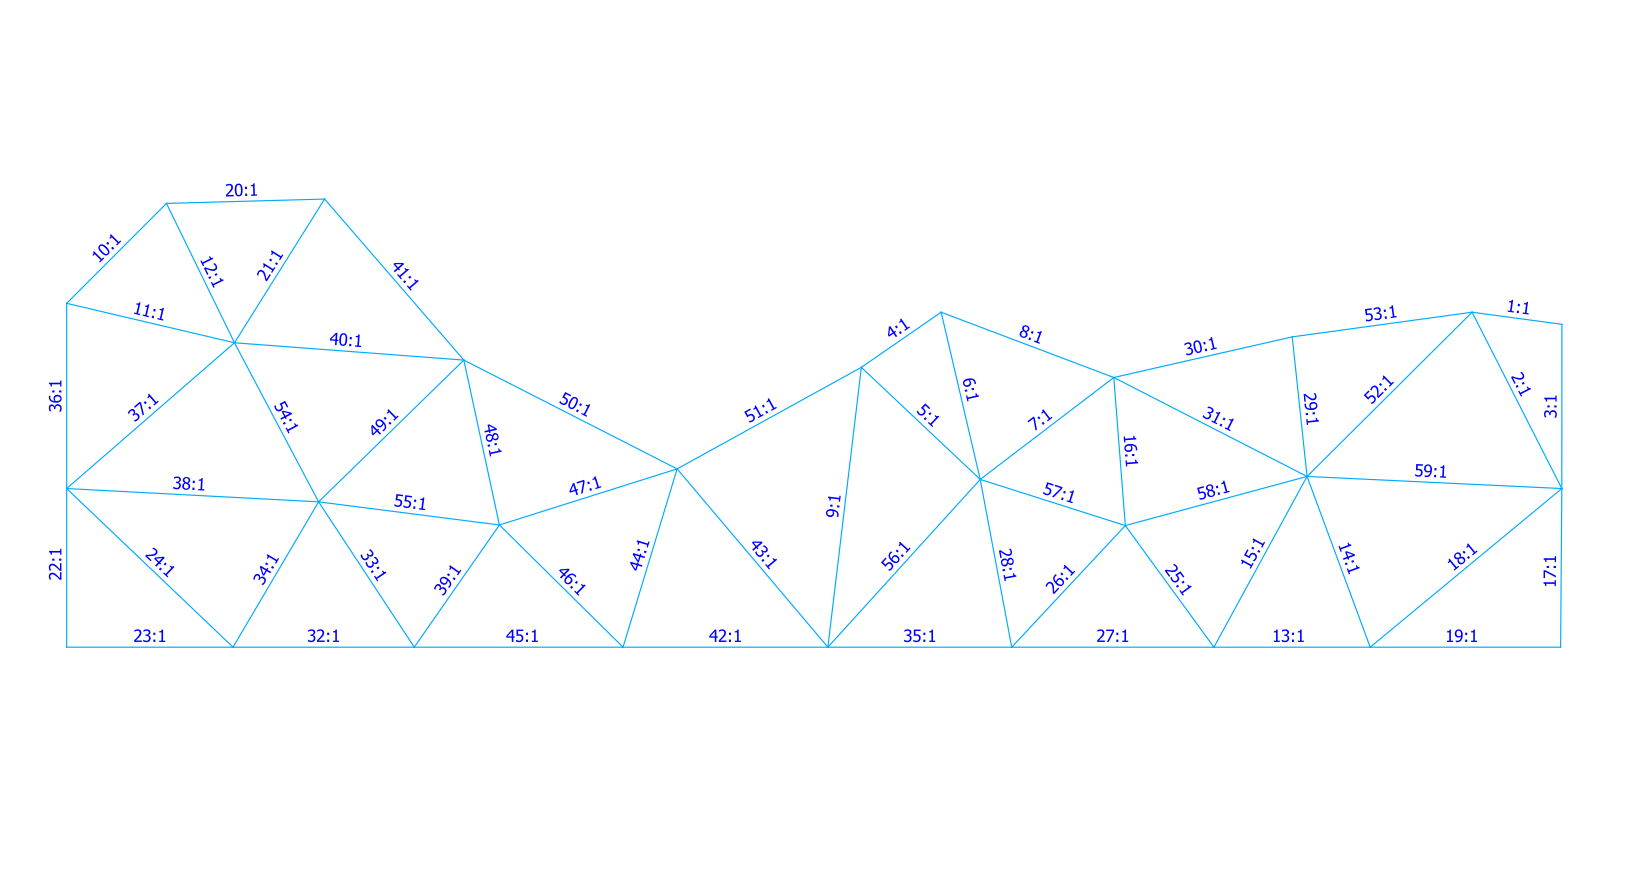
\includegraphics[width=0.8\textwidth]{pictures/edge_numbers_triangles.png}
	\caption{Edge numbers (1-based) of mesh consisting of only triangles}
\end{figure}
\begin{figure}[H]
	\centering
	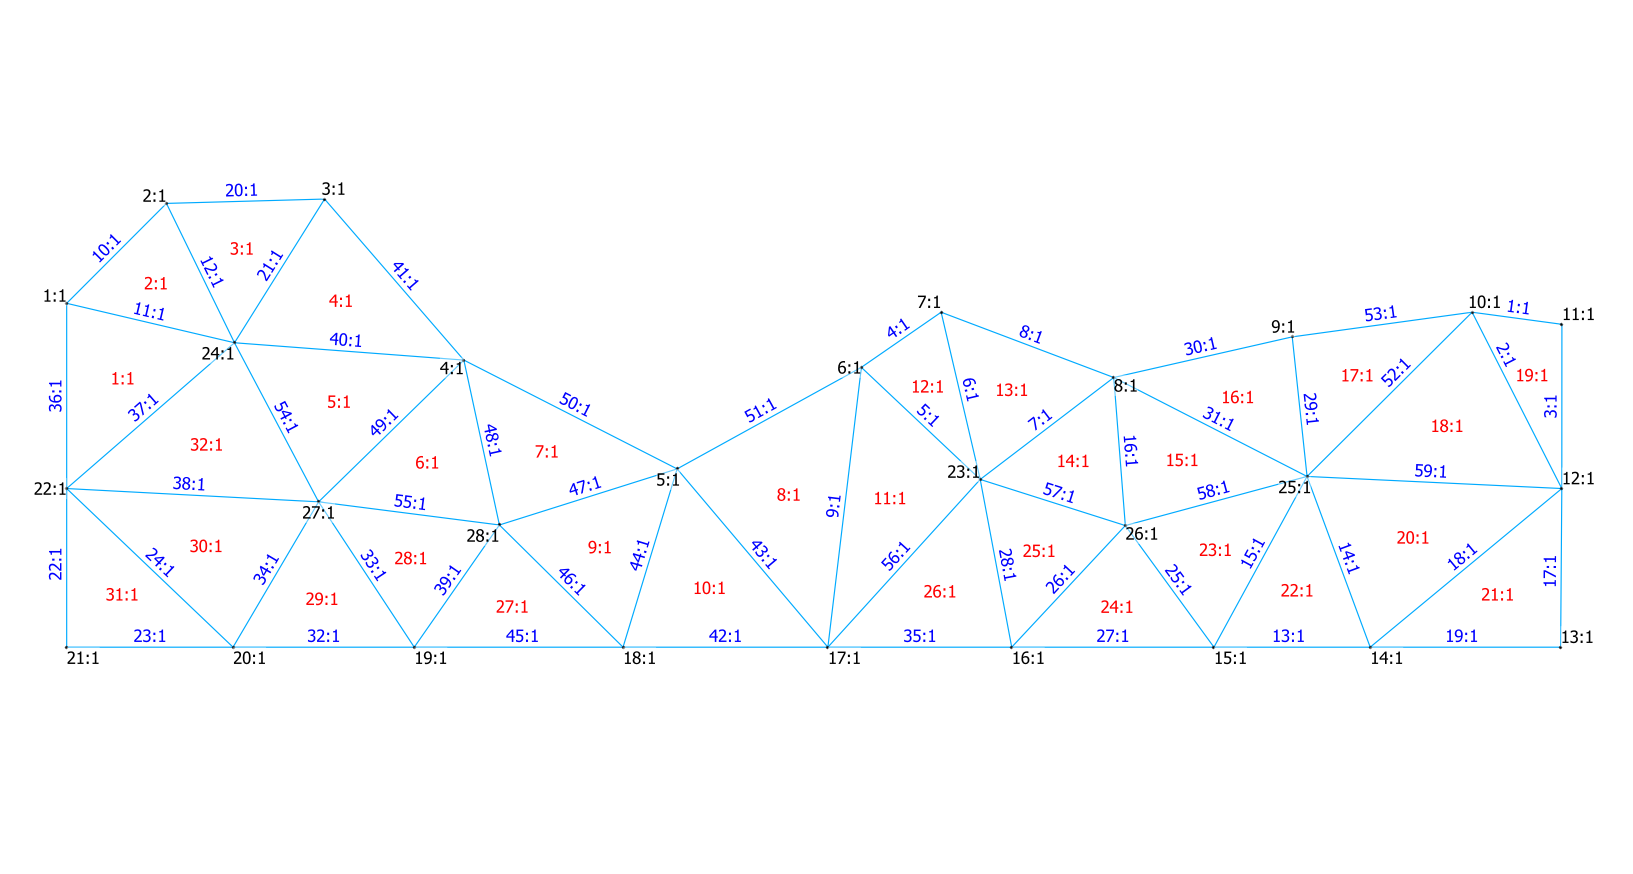
\includegraphics[width=0.8\textwidth]{pictures/all_numbers_triangles.png}
	\caption{Node, edge and face numbers (1-based) of mesh consisting of only triangles}
\end{figure}
%------------------------------------------------------------------------------
\section{Mesh consisting of triangles and quadrangles\label{sec:quadrangles}}
\begin{figure}[H]
	\centering
	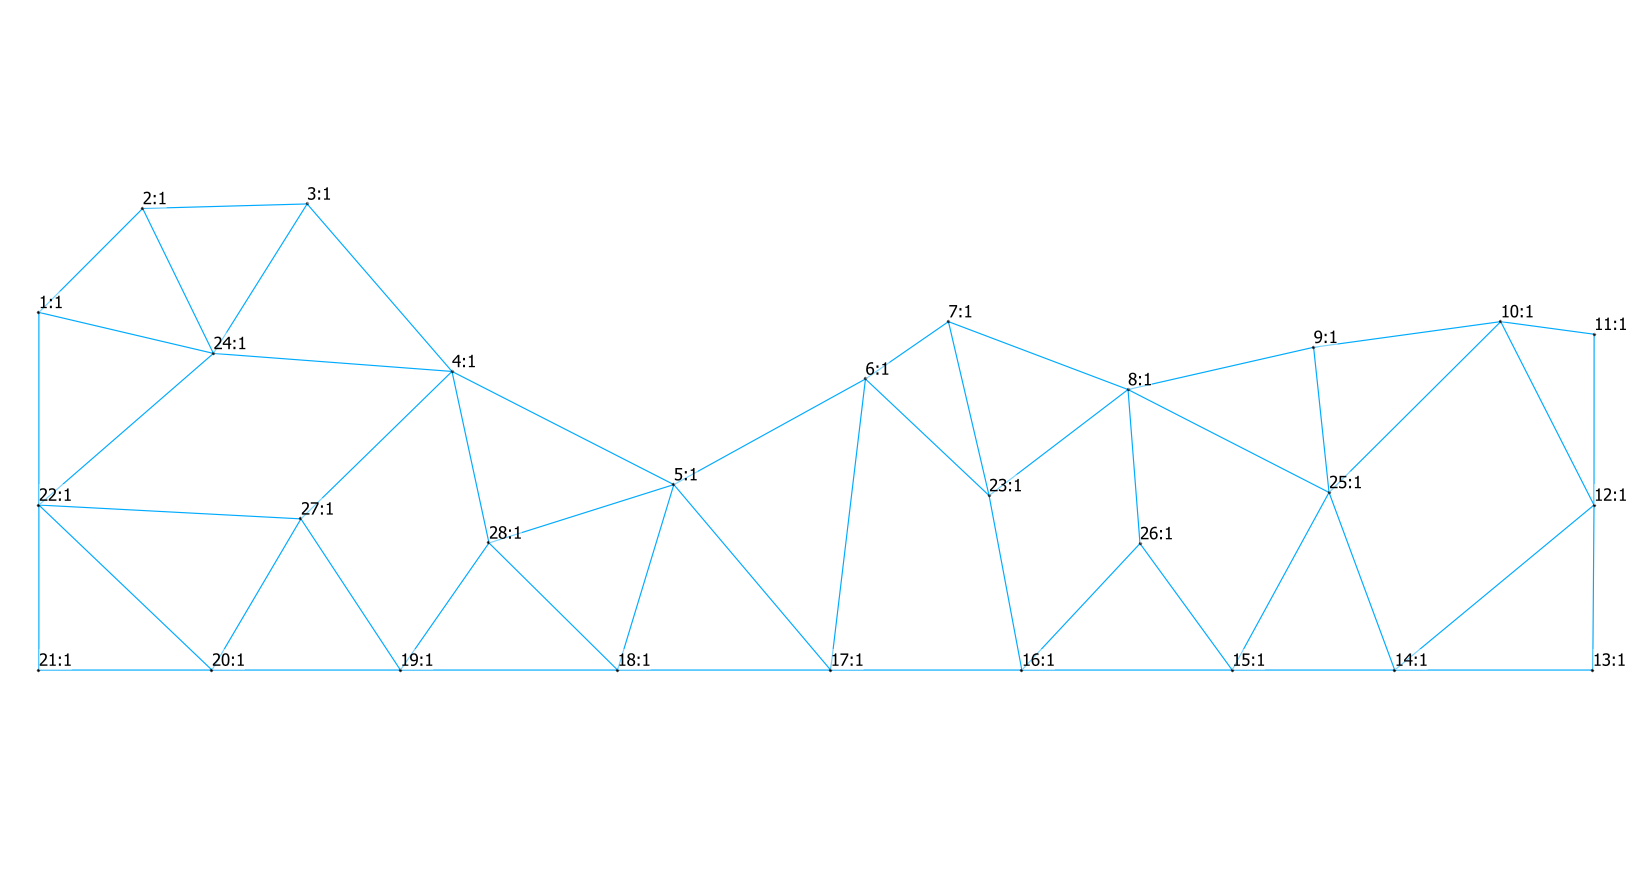
\includegraphics[width=0.8\textwidth]{pictures/node_numbers_quadrangles.png}
	\caption{Node numbers (1-based) of mesh consisting of triangles and quadrangles}
\end{figure}
\begin{figure}[H]
	\centering
	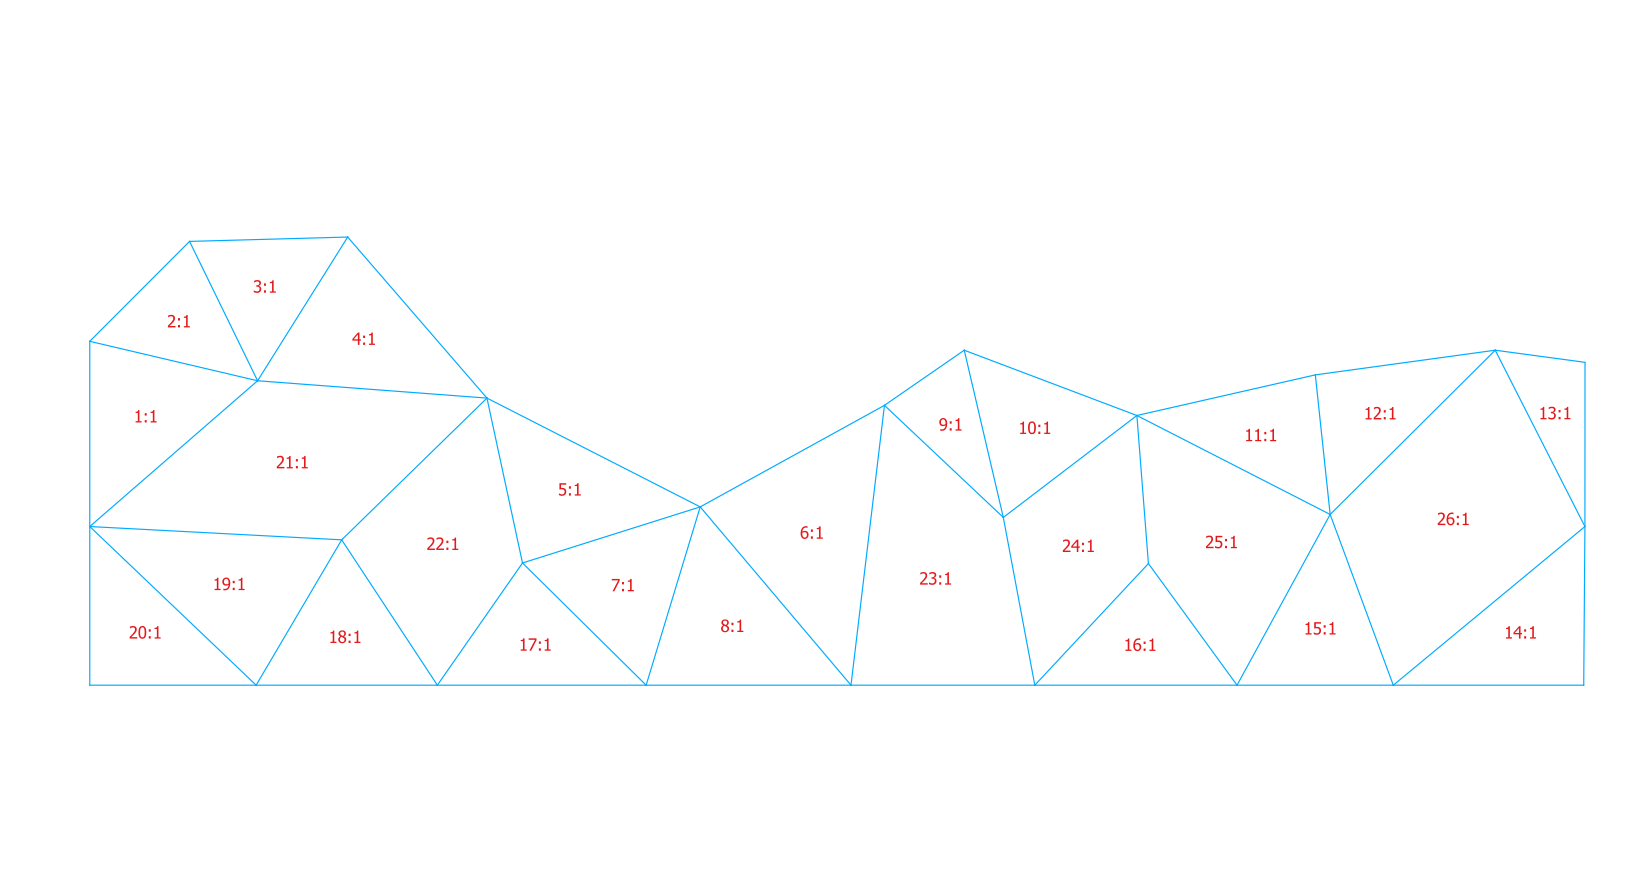
\includegraphics[width=0.8\textwidth]{pictures/face_numbers_quadrangles.png}
	\caption{Face numbers (1-based) of mesh consisting of triangles and quadrangles}
\end{figure}
\begin{figure}[H]
	\centering
	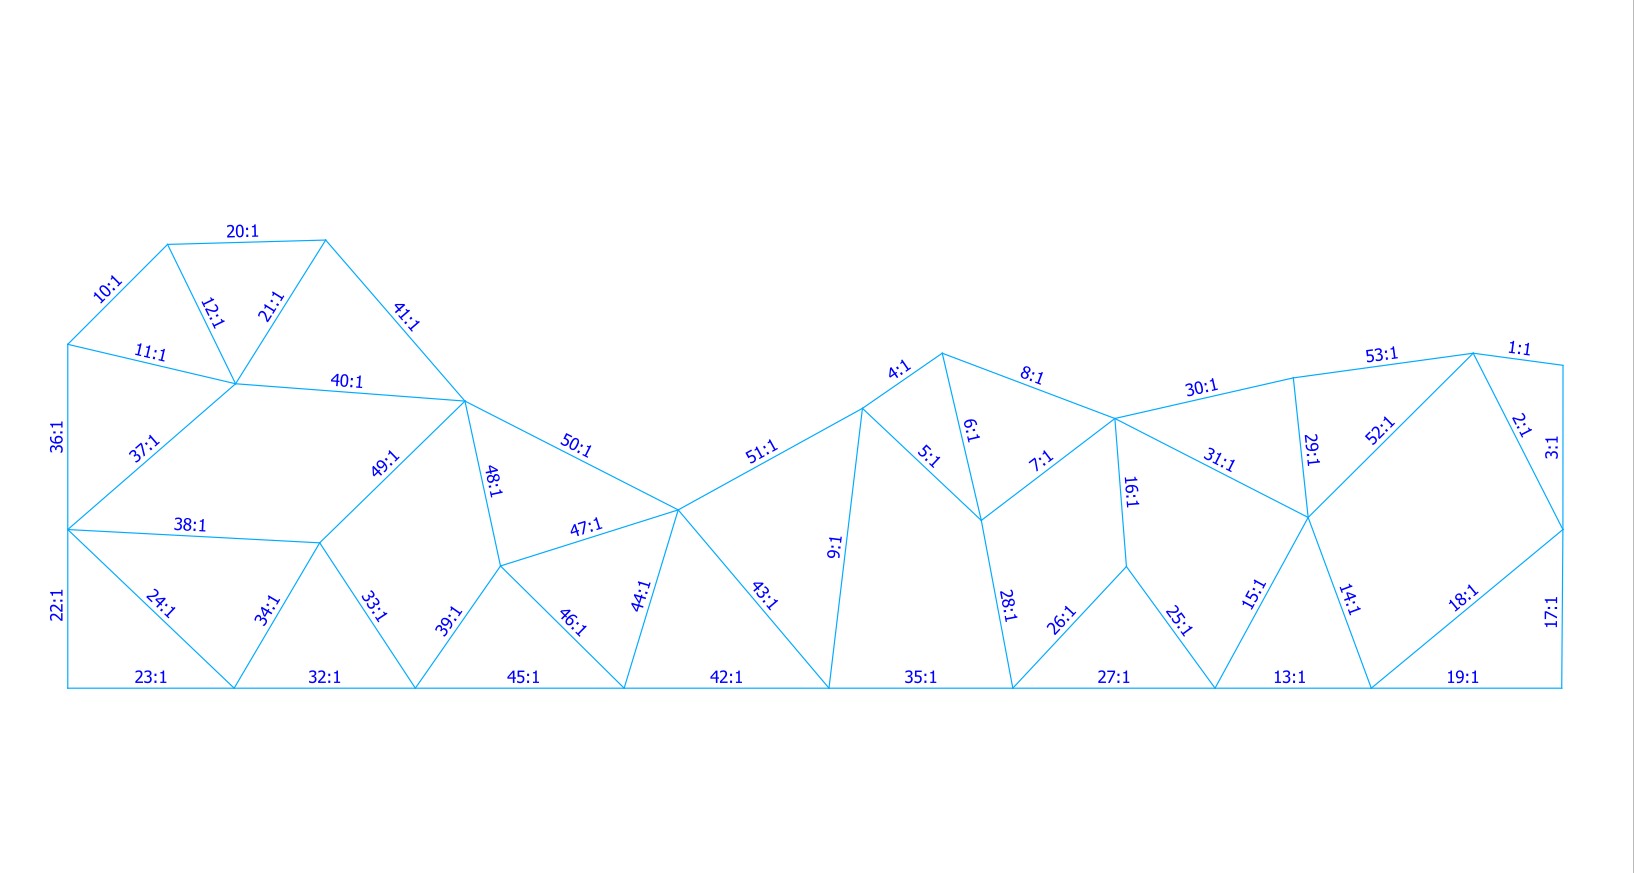
\includegraphics[width=0.8\textwidth]{pictures/edge_numbers_quadrangles.png}
	\caption{Edge numbers (1-based) of mesh consisting of triangles and quadrangles}
\end{figure}
\begin{figure}[H]
	\centering
	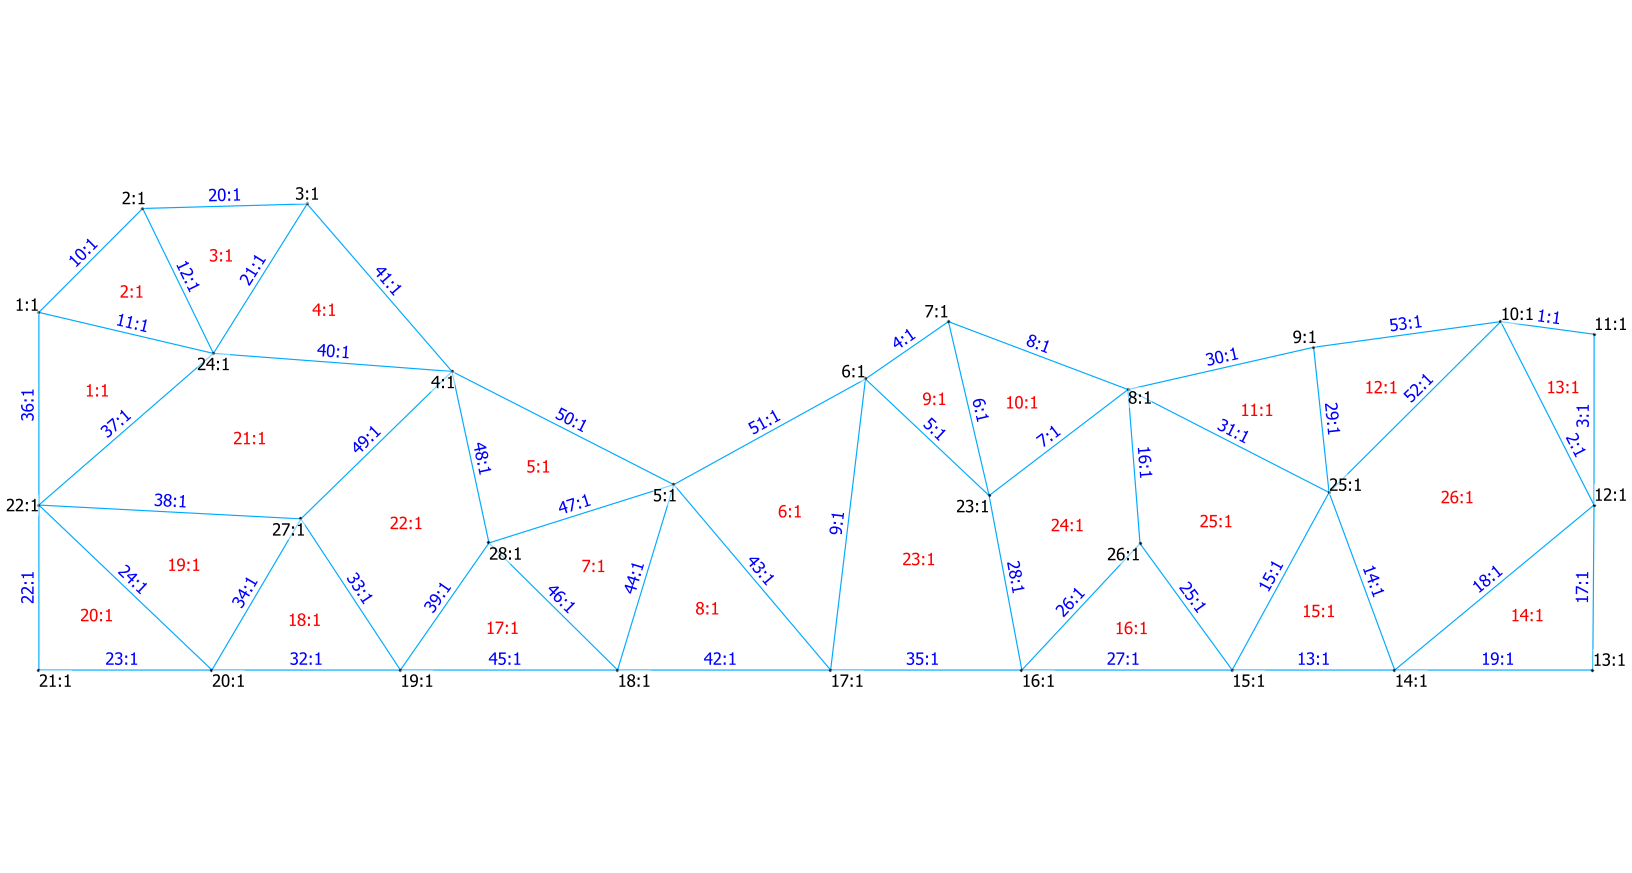
\includegraphics[width=0.8\textwidth]{pictures/all_numbers_quadrangles.png}
	\caption{Node, edge and face numbers (1-based) of mesh consisting of triangles and quadrangles}
\end{figure}

%------------------------------------------------------------------------------
\LastPage
\end{document}
